% !TeX root = ../../thesis.tex
\chapter{Enhancing Photodiode Performance Through Tailored Engineering of the Perovskite and Electron Transport Layer}\label{ch:transport_layer}


One of the most critical factors that indicates the performance of photodetectors is the dark current density (Jd), which constitutes the primary limitation on the device’s detectivity. Previous reports have shown that careful optimization of the ETL and HTL is critical for minimizing Jd in perovskite-based photodetectors. This was achieved by eliminating shunt pathways25, increasing the carrier injection barrier26,27, and preventing interfacial thermal charge generation28,29. However, most reports typically restrict the operational voltage range to approximately -0.5 V, despite the potential for higher carrier extraction speeds at greater reverse biases. This is because extensive reverse biasing of perovskite heterojunctions is known to have adverse effects on the device performance, including the risk of device breakdown. This manifests as a multiple-orders-of-magnitude increase in Jd and has been attributed to the creation of defect states in the perovskite bulk that act as charge recombination centers30. Specifically, it was shown that under reverse bias ions accumulate at the perovskite/ETL interface, facilitating the tunneling of holes into the perovskite bulk. Recombination centers are thereafter generated by the oxidation of halides to natural halogens31. Diffusion of iodine into the fullerene-based ETL was also shown to be an aftermath of reverse biasing32. Various breakdown mitigation strategies were proposed, including the introduction of a hole-blocking layer at perovskite/ETL interface33,34, the use of electrochemically inert electrodes34,35, as well as the deposition of thick planarizing polymer HTLs35. It is important to mention that all aforementioned studies focus on perovskite solar cells rather than photodetectors, where reverse biasing falls outside the “normal” operation conditions and may arise when a cell under shadow has to curry the current generated by the neighboring, illuminated cells.

\section{Benchmarking Photodiode Performance}

The first step in exploring device performance was selecting the transport layers for the PePD stack. The requirement for vacuum-deposited inorganic transport layers introduced several significant limitations. For the HTL, DC-sputtered \ch{NiO_x} was the only sufficiently mature option. However, due to the harsh conditions of the sputtering process, \ch{NiO_x} could only be deposited before the perovskite layer. For the ETL, the two most accessible candidates were e-beam deposited \ch{TiO_2} and thermally evaporated \ch{C_{60}}. Fig.~\ref{fig:ch2:tio2_compare} and Fig.~\ref{fig:ch2:c60_compare} compare the J-V scans of PePDs with \ch{TiO_2} and \ch{C_60} as the ETL, respectively. For each ETL, two versions of the stack were evaluated: one with an as-deposited perovskite layer and one with a flash-annealed perovskite layer. In the case of the annealed perovskite, annealing was performed before ETL deposition at 300 \degree C for 5–10 seconds in nitrogen environment. This was done considering that, while the as-deposited perovskite was already in the black phase, the annealed version exhibited higher crystallinity and improved optoelectronic properties, as discussed in the previous section.

\begin{figure}[htbp]
    \centering
    % First row
    \begin{subfigure}[t]{0.4\textwidth}
        \centering
        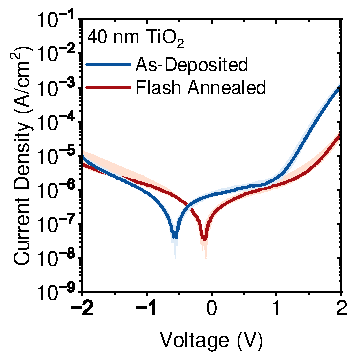
\includegraphics[width=\textwidth]{chapters/material_properties/images/TiO2-Compare.pdf} 
        \caption{}
        \label{fig:ch2:tio2_compare}
    \end{subfigure}
    \hfill
    \begin{subfigure}[t]{0.4\textwidth}
        \centering
        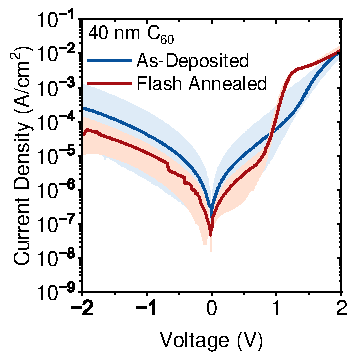
\includegraphics[width=\textwidth]{chapters/material_properties/images/C60-Compare.pdf} % Replace with your image file
        \caption{}
        \label{fig:ch2:c60_compare}
    \end{subfigure}


    % Second row
    \begin{subfigure}[t]{0.4\textwidth}
        \centering
        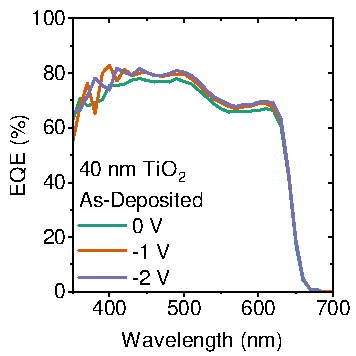
\includegraphics[width=\textwidth]{chapters/material_properties/images/As_Dep-EQE.pdf} % Replace with your image file
        \caption{}
        \label{fig:ch2:as_dep_eqe}
    \end{subfigure}
    \hfill
    \begin{subfigure}[t]{0.4\textwidth}
        \centering
        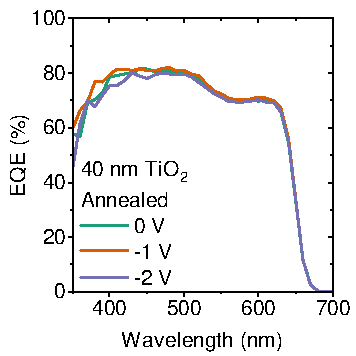
\includegraphics[width=\textwidth]{chapters/material_properties/images/Annealed_EQE.pdf} % Replace with your image file
        \caption{}
        \label{fig:ch2:annealed_eqe}
    \end{subfigure}
    \caption{Impact of transport layer and annealing conditions on device performance.}
\end{figure}

Both samples with \ch{TiO_2} exhibit similar levels of $J_d$ at -2 V, albeit the flash-annealed one has smaller hysteresis. The samples with \ch{C_60} exhibit significantly larger variability ans a median value of dark current at xx and yy for the as-deposited and annealed perovskite, respectively. Annealing the film seems to be reducing both the variability and the median value of dark current, however the performance is still superior compared to the samples with \ch{TiO_2}. It was previously shown that evaporated \ch{C_60} has the tendency to diffuse through the grain boundaries of the perovskite film, leading to potential shunts, and that is why it is mitigated with the annealing and larger grains. This phenomenon will be further investigated in Section xx. For this reason, for now we rely on the use of \ch{TiO_2} for the development of the baseline device stack. 

In terms of EQE for the \ch{TiO_2} samples, both exhibit a very similar behavior with an EQE that is already saturated at 0 V and is mainly above 70\% for the whole visible spectrum. These results further highlight the possibility of fabricating photodetectors processed solely at room temperature, a property that could open up new pathways for use with flexible substrates. However, considering the improvements in crystallinity and reduction in non-radiative recombination that were established for the annealed state, we move forward using the the flash-annealed sample with 40 nm of \ch{TiO_2} as the baseline. 



Beside the choice of transport layer and annealing of the perovskite, we wanted to explore the composition of the perovskite film, as well as the deposition speed on the performance. In terms of deposition rate we explore three deposition rates, ranging between 0.8, 1.2, and 1.6 {\AA}/sec. The overall performance is not drastically affected, however careful consideration of the $J_d$ at -2 V demonstrates an increase in the median value with faster deposition rate. Therefore, we maintain a deposition rate of 0.8 {\AA}/s for the rest of our experiments. 

In terms of stoichiometry, we vary the \ch{CsBr}:\ch{PbI_2} ratio between 0.8:1.0 (\ch{PbI_2} excess), 1.05:1.0 (Stoich), and 1.2:1.0 (\ch{CsBr} excess). For the samples with excess of \ch{PbI_2}, a significant overshoot is observed at the TPC measurement, typically associated with the accumulation of trapped charges at the interface, that limit the extraction of photo-generated carriers. Say something about sample with excess of CsBr...


\begin{figure}[htbp]
    \centering
    % First row
    \begin{subfigure}[t]{0.4\textwidth}
        \centering
        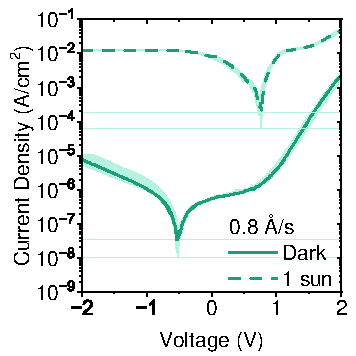
\includegraphics[width=\textwidth]{chapters/material_properties/images/08As-JV.pdf} 
        \caption{}
        \label{fig:ch2:0.8A/s-jv}
    \end{subfigure}
    \hfill
    \begin{subfigure}[t]{0.4\textwidth}
        \centering
        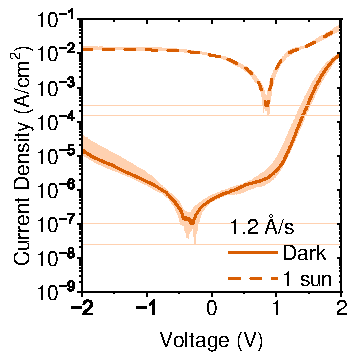
\includegraphics[width=\textwidth]{chapters/material_properties/images/12AS-JV.pdf} % Replace with your image file
        \caption{}
        \label{fig:ch2:1.2A/s-vj}
    \end{subfigure}

    % Second row
    \begin{subfigure}[t]{0.4\textwidth}
        \centering
        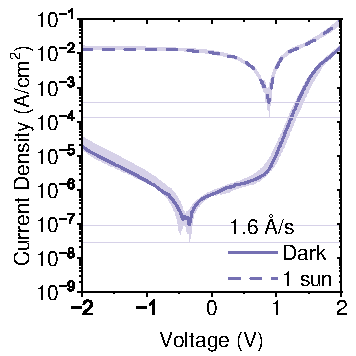
\includegraphics[width=\textwidth]{chapters/material_properties/images/16AS-JV.pdf} % Replace with your image file
        \caption{}
        \label{fig:ch2:1.6A/s-jv}
    \end{subfigure}
    \hfill
    \begin{subfigure}[t]{0.4\textwidth}
        \centering
        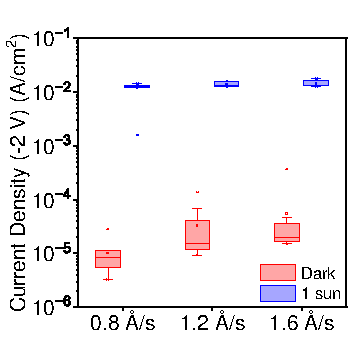
\includegraphics[width=\textwidth]{chapters/material_properties/images/Evap_Rate_Box_Plot.pdf} % Replace with your image file
        \caption{}
        \label{fig:ch2:box_plot_evap_rate}
    \end{subfigure}
    \caption{SSPL, TRPL, and absorptance for the an As-Deposited and an Annealed perovskite sample.}
\end{figure}




\begin{figure}[htbp]
    \centering

    % First row
    \begin{subfigure}[b]{0.3\textwidth}
        \centering
        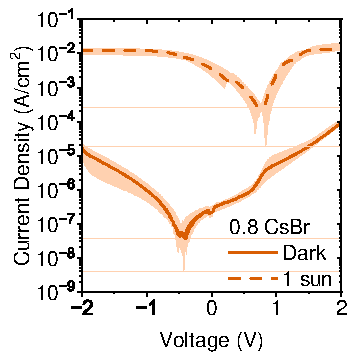
\includegraphics[width=\textwidth]{chapters/material_properties/images/08CsBr.pdf}
        \caption{}
    \end{subfigure}
    \hfill
    \begin{subfigure}[b]{0.3\textwidth}
        \centering
        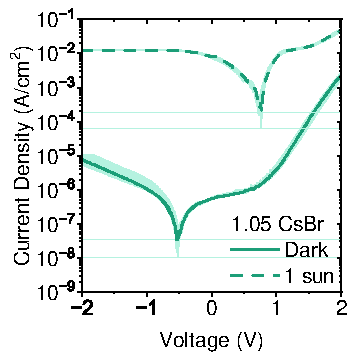
\includegraphics[width=\textwidth]{chapters/material_properties/images/105CsBr.pdf}
        \caption{}
    \end{subfigure}
    \hfill
    \begin{subfigure}[b]{0.3\textwidth}
        \centering
        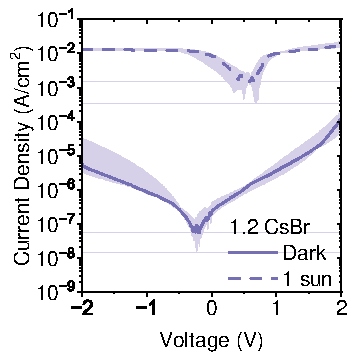
\includegraphics[width=\textwidth]{chapters/material_properties/images/12CsBr.pdf}
        \caption{}
    \end{subfigure}

    \vspace{1em} % Space between rows

    % Second row
    \begin{subfigure}[b]{0.28\textwidth}
        \centering
        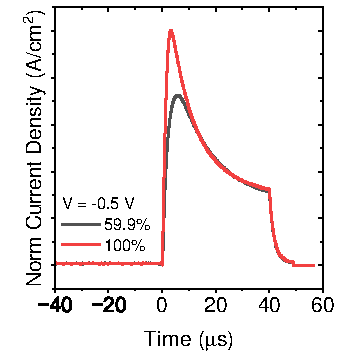
\includegraphics[width=\textwidth]{chapters/material_properties/images/TPC-08CsBr.pdf}
        \caption{}
    \end{subfigure}
    \hfill
    \begin{subfigure}[b]{0.28\textwidth}
        \centering
        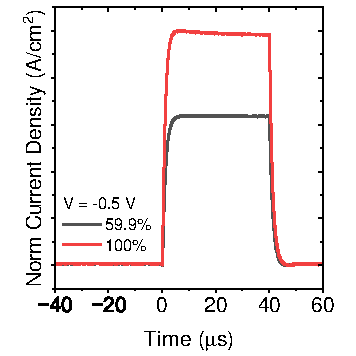
\includegraphics[width=\textwidth]{chapters/material_properties/images/TPC-105CsBr.pdf}
        \caption{}
    \end{subfigure}
    \hfill
    \begin{subfigure}[b]{0.28\textwidth}
        \centering
        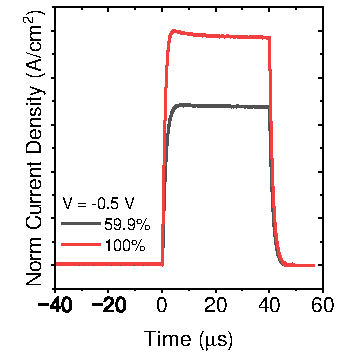
\includegraphics[width=\textwidth]{chapters/material_properties/images/tpc-12CsBr.pdf}
        \caption{}
    \end{subfigure}

    \caption{A figure with 2 rows and 3 images in each row.}
    \label{fig:two_rows_three_columns}
\end{figure}


\section{Electron Transport Optimization for Enhanced Reverse Bias Stability and Speed}


\begin{figure}[htbp]
    \centering
    \begin{subfigure}{0.24\textwidth}
        \centering
        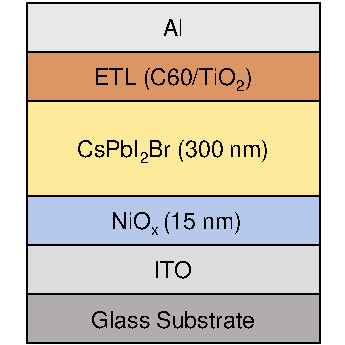
\includegraphics[width=\textwidth]{chapters/transport_layers/images/ETL_optimization_stack.pdf}
        \caption{}
        \label{}
    \end{subfigure}
    \hfill
    \begin{subfigure}{0.24\textwidth}
        \centering
        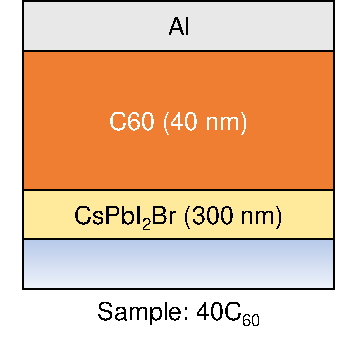
\includegraphics[width=\textwidth]{chapters/transport_layers/images/ETL_Optimization_40C60.pdf}
        \caption{}
        \label{}
    \end{subfigure}
    \hfill
    \begin{subfigure}{0.24\textwidth}
        \centering
        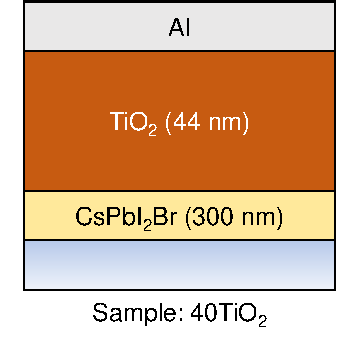
\includegraphics[width=\textwidth]{chapters/transport_layers/images/ETL_Optimization_40TiO2.pdf}
        \caption{}
        \label{}
    \end{subfigure}
    \hfill
    \begin{subfigure}{0.24\textwidth}
        \centering
        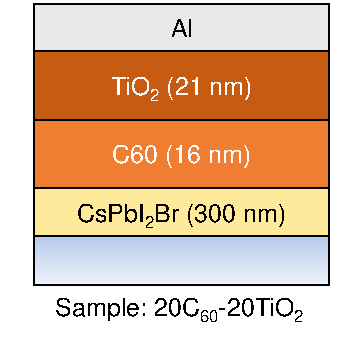
\includegraphics[width=\textwidth]{chapters/transport_layers/images/ETL_Optimization_20_20.pdf}
        \caption{}
        \label{}
    \end{subfigure}
    
    \caption{A 1×4 grid of images.}
    \label{}
\end{figure}




\begin{figure}[htbp]
    \centering

    % First row
    \begin{subfigure}[b]{0.32\textwidth}
        \centering
        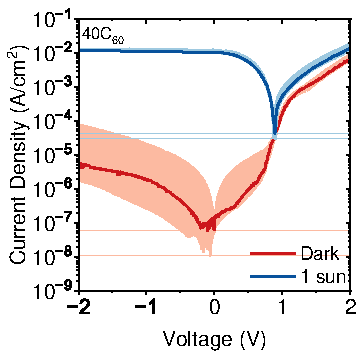
\includegraphics[width=\textwidth]{chapters/transport_layers/images/JV_Median_40C60.pdf}
        \caption{}
    \end{subfigure}
    \hfill
    \begin{subfigure}[b]{0.32\textwidth}
        \centering
        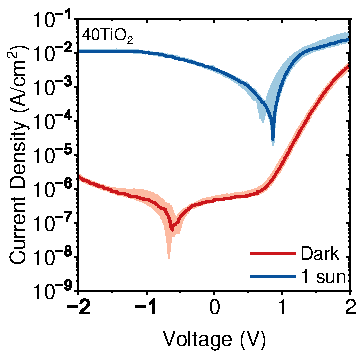
\includegraphics[width=\textwidth]{chapters/transport_layers/images/JV_Median_40TiO2.pdf}
        \caption{}
    \end{subfigure}
    \hfill
    \begin{subfigure}[b]{0.32\textwidth}
        \centering
        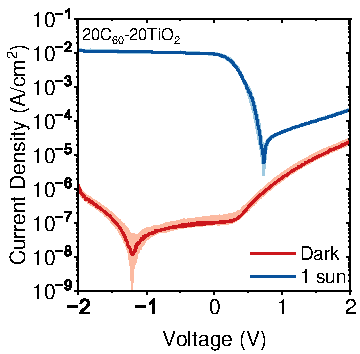
\includegraphics[width=\textwidth]{chapters/transport_layers/images/JV_Median_20_20.pdf}
        \caption{}
    \end{subfigure}

    \vspace{1em} % Space between rows

    % Second row
    \begin{subfigure}[b]{0.32\textwidth}
        \centering
        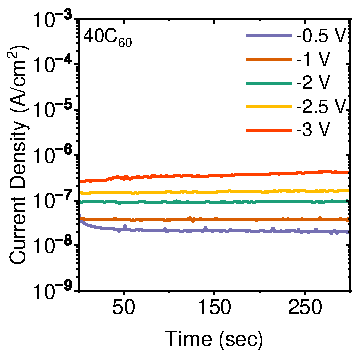
\includegraphics[width=\textwidth]{chapters/transport_layers/images/StaticJV_40C60.pdf}
        \caption{}
    \end{subfigure}
    \hfill
    \begin{subfigure}[b]{0.32\textwidth}
        \centering
        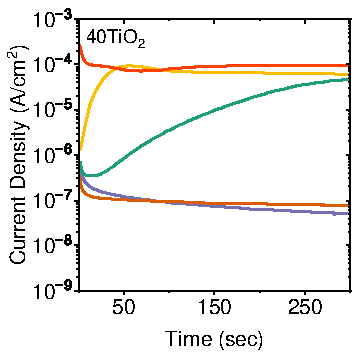
\includegraphics[width=\textwidth]{chapters/transport_layers/images/StaticJV_40TiO2.pdf}
        \caption{}
    \end{subfigure}
    \hfill
    \begin{subfigure}[b]{0.32\textwidth}
        \centering
        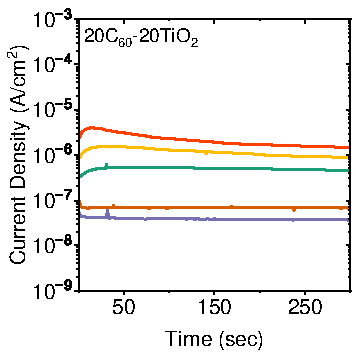
\includegraphics[width=\textwidth]{chapters/transport_layers/images/StaticJV_20_20.pdf}
        \caption{}
    \end{subfigure}

    \caption{A figure with 2 rows and 3 images in each row.}
    \label{fig:dicrete_and_static_jvs}
\end{figure}




\begin{figure}[htbp]
    \centering
    \begin{subfigure}{0.32\textwidth}
        \centering
        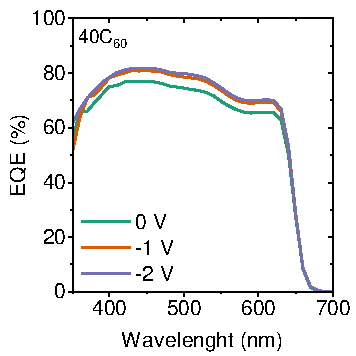
\includegraphics[width=\textwidth]{chapters/transport_layers/images/EQE_40C60.pdf}
        \caption{}
        \label{}
    \end{subfigure}
    \hfill
    \begin{subfigure}{0.32\textwidth}
        \centering
        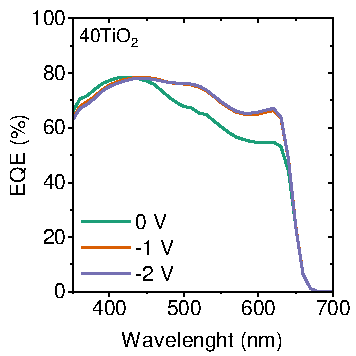
\includegraphics[width=\textwidth]{chapters/transport_layers/images/EQE_40TiO2.pdf}
        \caption{}
        \label{}
    \end{subfigure}
    \hfill
    \begin{subfigure}{0.32\textwidth}
        \centering
        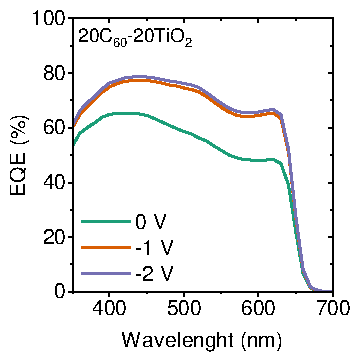
\includegraphics[width=\textwidth]{chapters/transport_layers/images/EQE_20_20.pdf}
        \caption{}
        \label{}
    \end{subfigure}
    
    \caption{A 1×3 grid of images.}
    \label{}
\end{figure}


\begin{figure}[htbp]
    \centering
    % First plot
    \begin{subfigure}[t]{0.45\textwidth} % Adjust width as needed
        \centering
        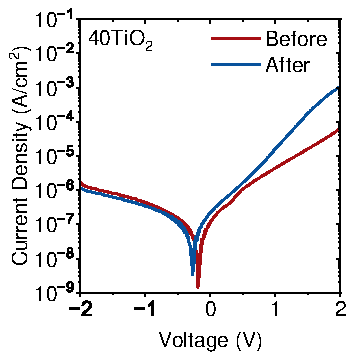
\includegraphics[width=\textwidth]{chapters/transport_layers/images/JV_Before_After_40TiO2.pdf} % Replace with your image
        \caption{}
        \label{}
    \end{subfigure}
    \hfill % Space between the two plots
    % Second plot
    \begin{subfigure}[t]{0.49\textwidth} % Adjust width as needed
        \centering
        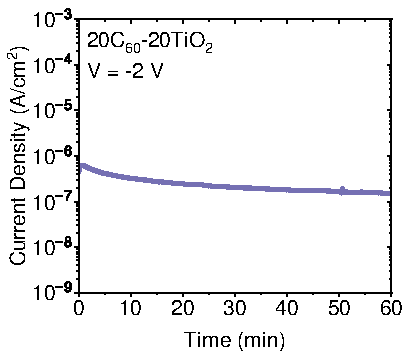
\includegraphics[width=\textwidth]{chapters/transport_layers/images/JV_1hr_20_20.pdf} % Replace with your image
        \caption{}
        \label{}
    \end{subfigure}

    % Caption for the whole figure
    \caption{Reversibility and long bias}
    \label{}
\end{figure}


\begin{figure}[htbp]
    \centering
    \begin{subfigure}{0.32\textwidth}
        \centering
        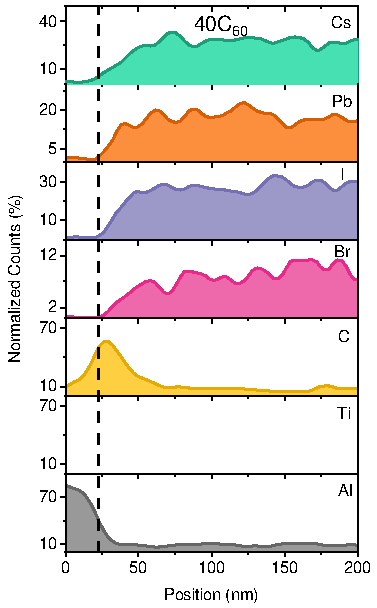
\includegraphics[width=\textwidth]{chapters/transport_layers/images/TEM_40C60.pdf}
        \caption{}
        \label{}
    \end{subfigure}
    \hfill
    \begin{subfigure}{0.32\textwidth}
        \centering
        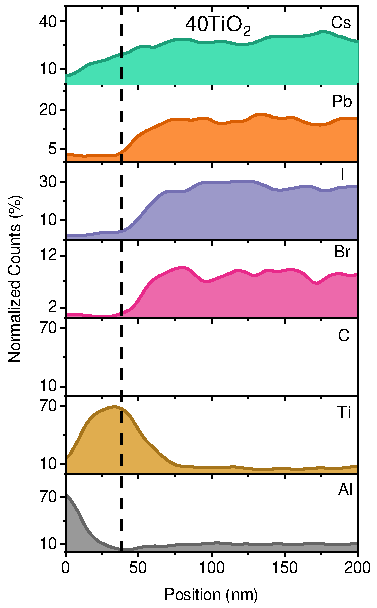
\includegraphics[width=\textwidth]{chapters/transport_layers/images/TEM_40TiO2.pdf}
        \caption{}
        \label{}
    \end{subfigure}
    \hfill
    \begin{subfigure}{0.32\textwidth}
        \centering
        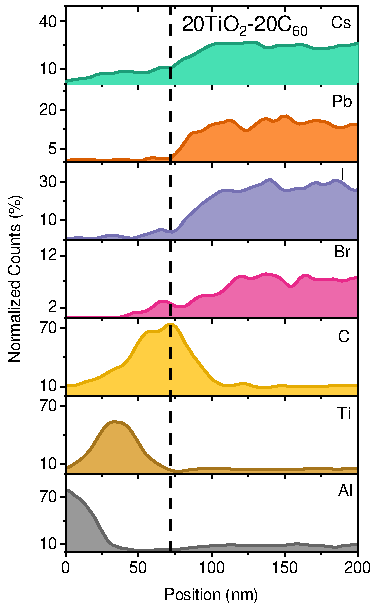
\includegraphics[width=\textwidth]{chapters/transport_layers/images/TEM_20_20.pdf}
        \caption{}
        \label{}
    \end{subfigure}
    
    \caption{A 1×3 grid of images.}
    \label{}
\end{figure}


\begin{figure}[htbp]
    \centering
    \begin{subfigure}{0.32\textwidth}
        \centering
        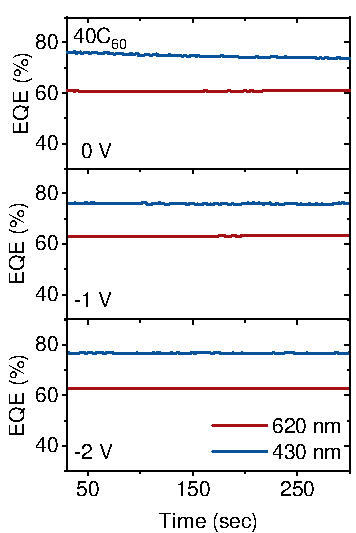
\includegraphics[width=\textwidth]{chapters/transport_layers/images/StaticEQE_40C60.pdf}
        \caption{}
        \label{}
    \end{subfigure}
    \hfill
    \begin{subfigure}{0.32\textwidth}
        \centering
        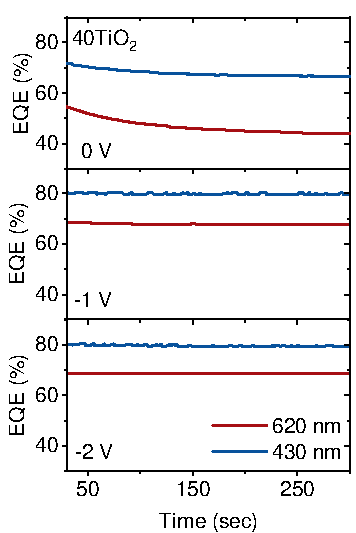
\includegraphics[width=\textwidth]{chapters/transport_layers/images/StaticEQE_40TiO2.pdf}
        \caption{}
        \label{}
    \end{subfigure}
    \hfill
    \begin{subfigure}{0.32\textwidth}
        \centering
        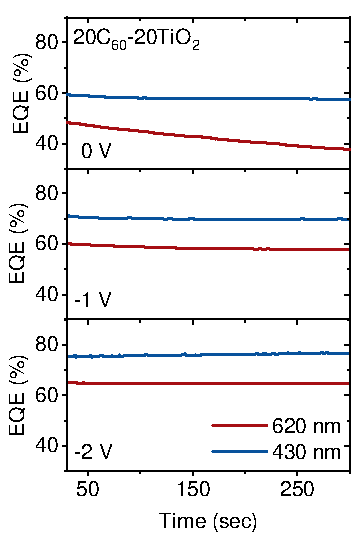
\includegraphics[width=\textwidth]{chapters/transport_layers/images/StaticEQE_20_20.pdf}
        \caption{}
        \label{}
    \end{subfigure}
    
    \caption{A 1×3 grid of images.}
    \label{}
\end{figure}



\begin{figure}[htbp]
    \centering
    \begin{subfigure}{0.245\textwidth}
        \centering
        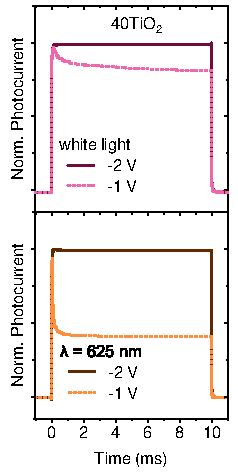
\includegraphics[width=\textwidth]{chapters/transport_layers/images/TPC_40TiO2.pdf}
        \caption{}
        \label{}
    \end{subfigure}
    \hfill
    \begin{subfigure}{0.245\textwidth}
        \centering
        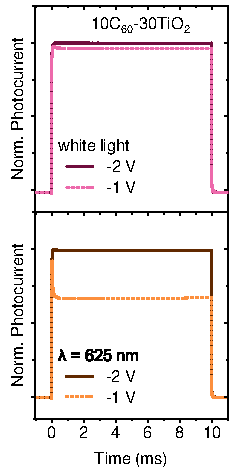
\includegraphics[width=\textwidth]{chapters/transport_layers/images/TPC_10_30.pdf}
        \caption{}
        \label{}
    \end{subfigure}
    \hfill
    \begin{subfigure}{0.245\textwidth}
        \centering
        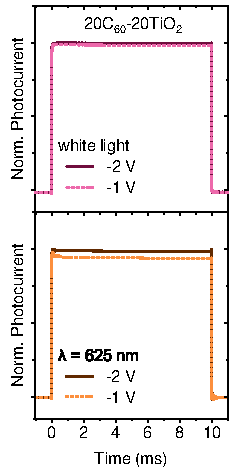
\includegraphics[width=\textwidth]{chapters/transport_layers/images/TPC_20_20.pdf}
        \caption{}
        \label{}
    \end{subfigure}
    \hfill
    \begin{subfigure}{0.245\textwidth}
        \centering
        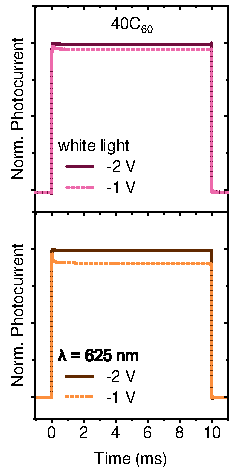
\includegraphics[width=\textwidth]{chapters/transport_layers/images/TPC_40C60.pdf}
        \caption{}
        \label{}
    \end{subfigure}
    
    \caption{A 1×4 grid of images.}
    \label{}
\end{figure}



\begin{figure}[t]
    \centering
    % First row
    \begin{subfigure}[t]{0.45\textwidth}
        \centering
        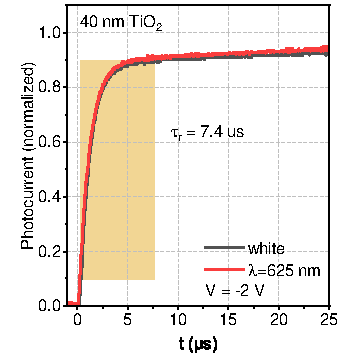
\includegraphics[width=\textwidth]{chapters/transport_layers/images/Rise_time_40TiO2.pdf} % Replace with your image file
        \caption{}
        \label{}
    \end{subfigure}
    \hfill
    \begin{subfigure}[t]{0.45\textwidth}
        \centering
        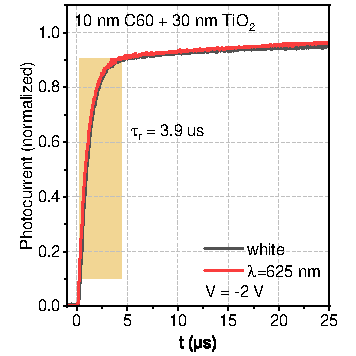
\includegraphics[width=\textwidth]{chapters/transport_layers/images/Rise_time_10_30.pdf} 
        % Replace with your image file
        \caption{}
        \label{}
    \end{subfigure} 
 % Second row
    \begin{subfigure}[t]{0.45\textwidth}
        \centering
        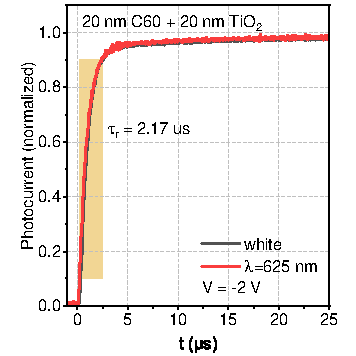
\includegraphics[width=\textwidth]{chapters/transport_layers/images/Rise_time_20_20.pdf} % Replace with your image file
        \caption{}
        \label{}
    \end{subfigure}
    \hfill
    \begin{subfigure}[t]{0.45\textwidth}
        \centering
        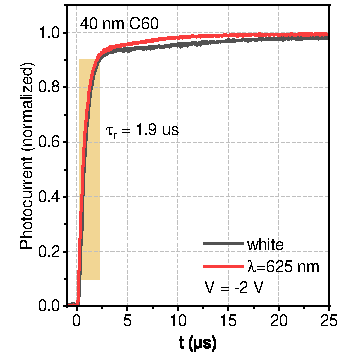
\includegraphics[width=\textwidth]{chapters/transport_layers/images/Rise_time_40C60.pdf} % Replace with your image file
        \caption{}
        \label{}
    \end{subfigure}
    \caption{}
    \label{}
\end{figure}



\begin{figure}[t]
    \centering
    % First row
    \begin{subfigure}[t]{0.45\textwidth}
        \centering
        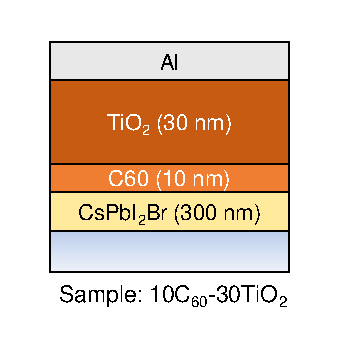
\includegraphics[width=\textwidth]{chapters/transport_layers/images/Sample_10_30_icon.pdf} % Replace with your image file
        \caption{}
        \label{}
    \end{subfigure}
    \hfill
    \begin{subfigure}[t]{0.45\textwidth}
        \centering
        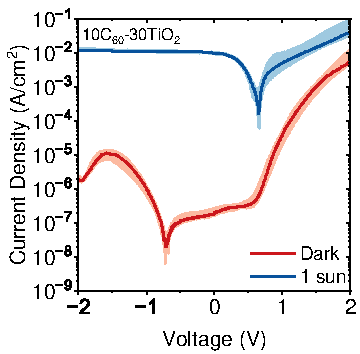
\includegraphics[width=\textwidth]{chapters/transport_layers/images/JV_Median_10_30.pdf} 
        % Replace with your image file
        \caption{}
        \label{}
    \end{subfigure} 
 % Second row
    \begin{subfigure}[t]{0.45\textwidth}
        \centering
        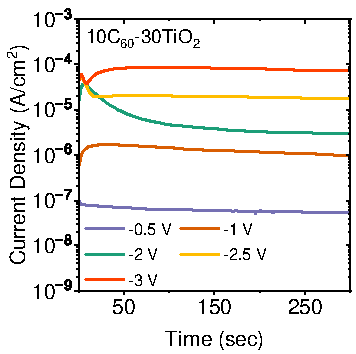
\includegraphics[width=\textwidth]{chapters/transport_layers/images/StaticJV_10_30.pdf} % Replace with your image file
        \caption{}
        \label{}
    \end{subfigure}
    \hfill
    \begin{subfigure}[t]{0.45\textwidth}
        \centering
        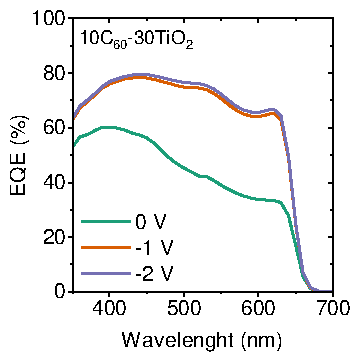
\includegraphics[width=\textwidth]{chapters/transport_layers/images/EQE_10_30.pdf} % Replace with your image file
        \caption{}
        \label{}
    \end{subfigure}
    \caption{}
    \label{}
\end{figure}


\begin{figure}[t]
    \centering
    % First row
    \begin{subfigure}[t]{0.45\textwidth}
        \centering
        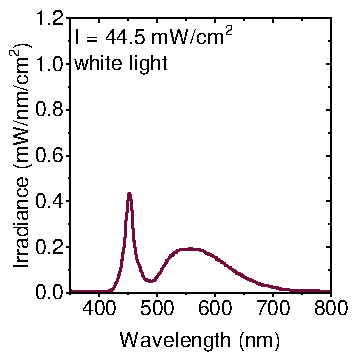
\includegraphics[width=\textwidth]{chapters/transport_layers/images/white_led.pdf} % Replace with your image file
        \caption{}
        \label{}
    \end{subfigure}
    \hfill
    \begin{subfigure}[t]{0.45\textwidth}
        \centering
        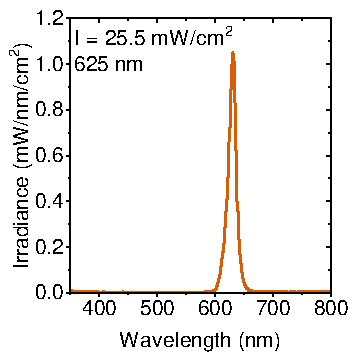
\includegraphics[width=\textwidth]{chapters/transport_layers/images/red_led.pdf} 
        % Replace with your image file
        \caption{}
        \label{}
    \end{subfigure} 
 % Second row
    \begin{subfigure}[t]{0.45\textwidth}
        \centering
        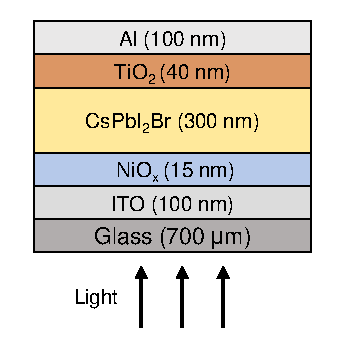
\includegraphics[width=\textwidth]{chapters/transport_layers/images/transfer_matrix_model.pdf} % Replace with your image file
        \caption{}
        \label{}
    \end{subfigure}
    \hfill
    \begin{subfigure}[t]{0.45\textwidth}
        \centering
        \includegraphics[width=\textwidth]{chapters/transport_layers/images/Generation_Rate.pdf} % Replace with your image file
        \caption{}
        \label{}
    \end{subfigure}
    \caption{}
    \label{}
\end{figure}


\begin{figure}[htbp]
    \centering
    % First plot
    \begin{subfigure}[t]{0.42\textwidth} % Adjust width as needed
        \centering
        \includegraphics[width=\textwidth]{chapters/transport_layers/images/MOS_Structure_icon.pdf} % Replace with your image
        \caption{}
        \label{}
    \end{subfigure}
    \hfill % Space between the two plots
    % Second plot
    \begin{subfigure}[t]{0.45\textwidth} % Adjust width as needed
        \centering
        \includegraphics[width=\textwidth]{chapters/transport_layers/images/MOS_IS.pdf} % Replace with your image
        \caption{}
        \label{}
    \end{subfigure}

    % Caption for the whole figure
    \caption{Reversibility and long bias}
    \label{}
\end{figure}


\begin{figure}[t]
    \centering
    % First row
    \begin{subfigure}[t]{0.42\textwidth}
        \centering
        \includegraphics[width=\textwidth]{chapters/transport_layers/images/TPC_comparison.pdf} % Replace with your image file
        \caption{}
        \label{}
    \end{subfigure}
    \hfill
    \begin{subfigure}[t]{0.4\textwidth}
        \centering
        \includegraphics[width=\textwidth]{chapters/transport_layers/images/Rise_time_f_c60_thickness.pdf} 
        % Replace with your image file
        \caption{}
        \label{}
    \end{subfigure} 
 % Second row
    \begin{subfigure}[t]{0.48\textwidth}
        \centering
        \hspace{-1.5cm}
        \includegraphics[width=\textwidth]{chapters/transport_layers/images/Cf_comparison.pdf} % Replace with your image file
        \caption{}
        \label{}
    \end{subfigure}
    \hfill
    \begin{subfigure}[t]{0.45\textwidth}
        \centering
        \includegraphics[width=\textwidth]{chapters/transport_layers/images/C_f_c60_thick.pdf} % Replace with your image file
        \caption{}
        \label{}
    \end{subfigure}
    \caption{}
    \label{}
\end{figure}


\begin{figure}[htbp]
    \centering
    \begin{subfigure}{0.32\textwidth}
        \centering
        \includegraphics[width=\textwidth]{chapters/transport_layers/images/Cf_40C60.pdf}
        \caption{}
        \label{}
    \end{subfigure}
    \hfill
    \begin{subfigure}{0.32\textwidth}
        \centering
        \includegraphics[width=\textwidth]{chapters/transport_layers/images/Cf_40TiO2.pdf}
        \caption{}
        \label{}
    \end{subfigure}
    \hfill
    \begin{subfigure}{0.32\textwidth}
        \centering
        \includegraphics[width=\textwidth]{chapters/transport_layers/images/Cf_20_20.pdf}
        \caption{}
        \label{}
    \end{subfigure}
    
    \caption{A 1×3 grid of images.}
    \label{}
\end{figure}



\begin{figure}[htbp]
    \centering
    \begin{subfigure}{0.35\textwidth}
        \centering
        \includegraphics[width=\textwidth]{chapters/transport_layers/images/Capacitance_f_area.pdf}
        \caption{}
        \label{}
    \end{subfigure}
    \hfill
    \begin{subfigure}{0.3\textwidth}
        \centering
        \includegraphics[width=\textwidth]{chapters/transport_layers/images/TPC_f_area.pdf}
        \caption{}
        \label{}
    \end{subfigure}
    \hfill
    \begin{subfigure}{0.29\textwidth}
        \centering
        \includegraphics[width=\textwidth]{chapters/transport_layers/images/Rise_time_farea.pdf}
        \caption{}
        \label{}
    \end{subfigure}
    
    \caption{A 1×3 grid of images.}
    \label{}
\end{figure}



\section{Conclusions}

Perovskite are known for their defect tolerant structure, this means that variation from the perfect stoichiometry do not have a negative impact on the performance of the device. This has an opposite effect at the same time, that despite pursuing changes in the composition and the fabrication does not translate to a major impact on the the device performance. 


%%%%%%%%%%%%%%%%%%%%%%%%%%%%%%%%%%%%%%%%%%%%%%%%%%
% Keep the following \cleardoublepage at the end of this file, 
% otherwise \includeonly includes empty pages.
\cleardoublepage

